\subsection{Results}
The robot scans the entire freespace, detecting all 287 cups.
All cups are picked up and returned to the offloading stations.
The total traveled path length is 36918.9 m, corresponding to a travel time of 7 hours and 24 minutes.

Figure \ref{cup_collection_results} shows part of the offline generated map vs. the traveled path in the same part of the map.

\begin{figure}[ht]
\centering
  \begin{subfigure}[t]{0.3\textwidth}
    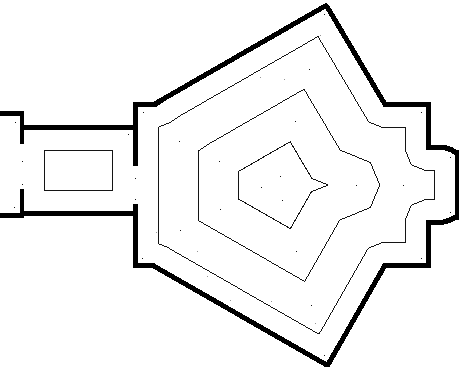
\includegraphics[width = \textwidth]{graphics/cup_collect_plan}
    \caption{Part of the offline generated map for cup collection. The coordinates in \(S_{M}\) are marked.}
    \label{cup_collect_plan}
  \end{subfigure}
  \begin{subfigure}[t]{0.3\textwidth}
    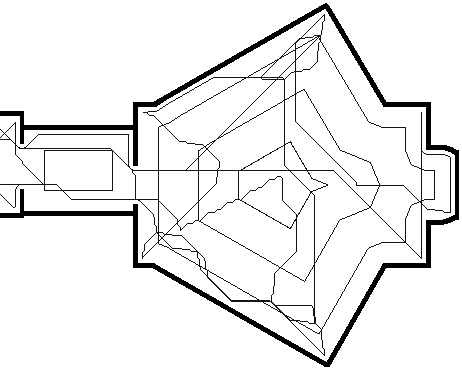
\includegraphics[width = \textwidth]{graphics/cup_collect_robot}
    \caption{Part of the traveled path in cup collection. The coordinates visited are marked.}
    \label{cup_collect_robot}
  \end{subfigure}
\caption{Cup collection planned vs. traveled}
\label{cup_collection_results}
\end{figure}